% !TeX root = ../SPL-Rules.tex
% !TeX spellcheck = en_US
\section{Technical Challenges}

\subsection{7 vs. 7}
    This competition extends the ideas from the mixed team competition, and 1 vs. 1 remote challenge from RoboCup 2021 to a standardized 7 vs. 7 on-site competition. Another goal is to enforce more collaborative game play. This challenge will only be executed if at least four teams participate.

    \subsubsection{Condition for participation}
    \label{sec:7vs7:condition_for_participation}
        \begin{itemize}
            \item A 7 vs. 7 team can be build from a single team but also from multiple teams.
            \item Teams need at least four own robots to play with.
            \item Teams have to provide three tested robots (\textbf{only V6 version}) to a robot pool.
            \item The pool robots have to be calibrated in limited time.
        \end{itemize}

    \subsubsection{Rules}
        This challenge bases on all rules from the 5 vs. 5 competition (\crefrange{sec:setup_environment}{sec:judgment}). The following list contains extended and changed rules for this challenge in order to ensure, among other things, the safety of pool robots:

        \paragraph{Players}
            In total each team consists of 7 players without a substitution robot. The 7 robots consist of 4 own and 3 pool robots. Whereby the pool robots are only V6s. Each jersey shirt has therefore now player numbers between 1 and 7 printed on it (\cf \cref{sec:team_markers}). Also the new positions of the initial kick-off (\cf \cref{sec:initial-kick-off}) for 7 robots can be seen in \cref{fig:initial_positions_7vs7}.
            \begin{figure}[t!]
            	\begin{center}
            		\leavevmode
            		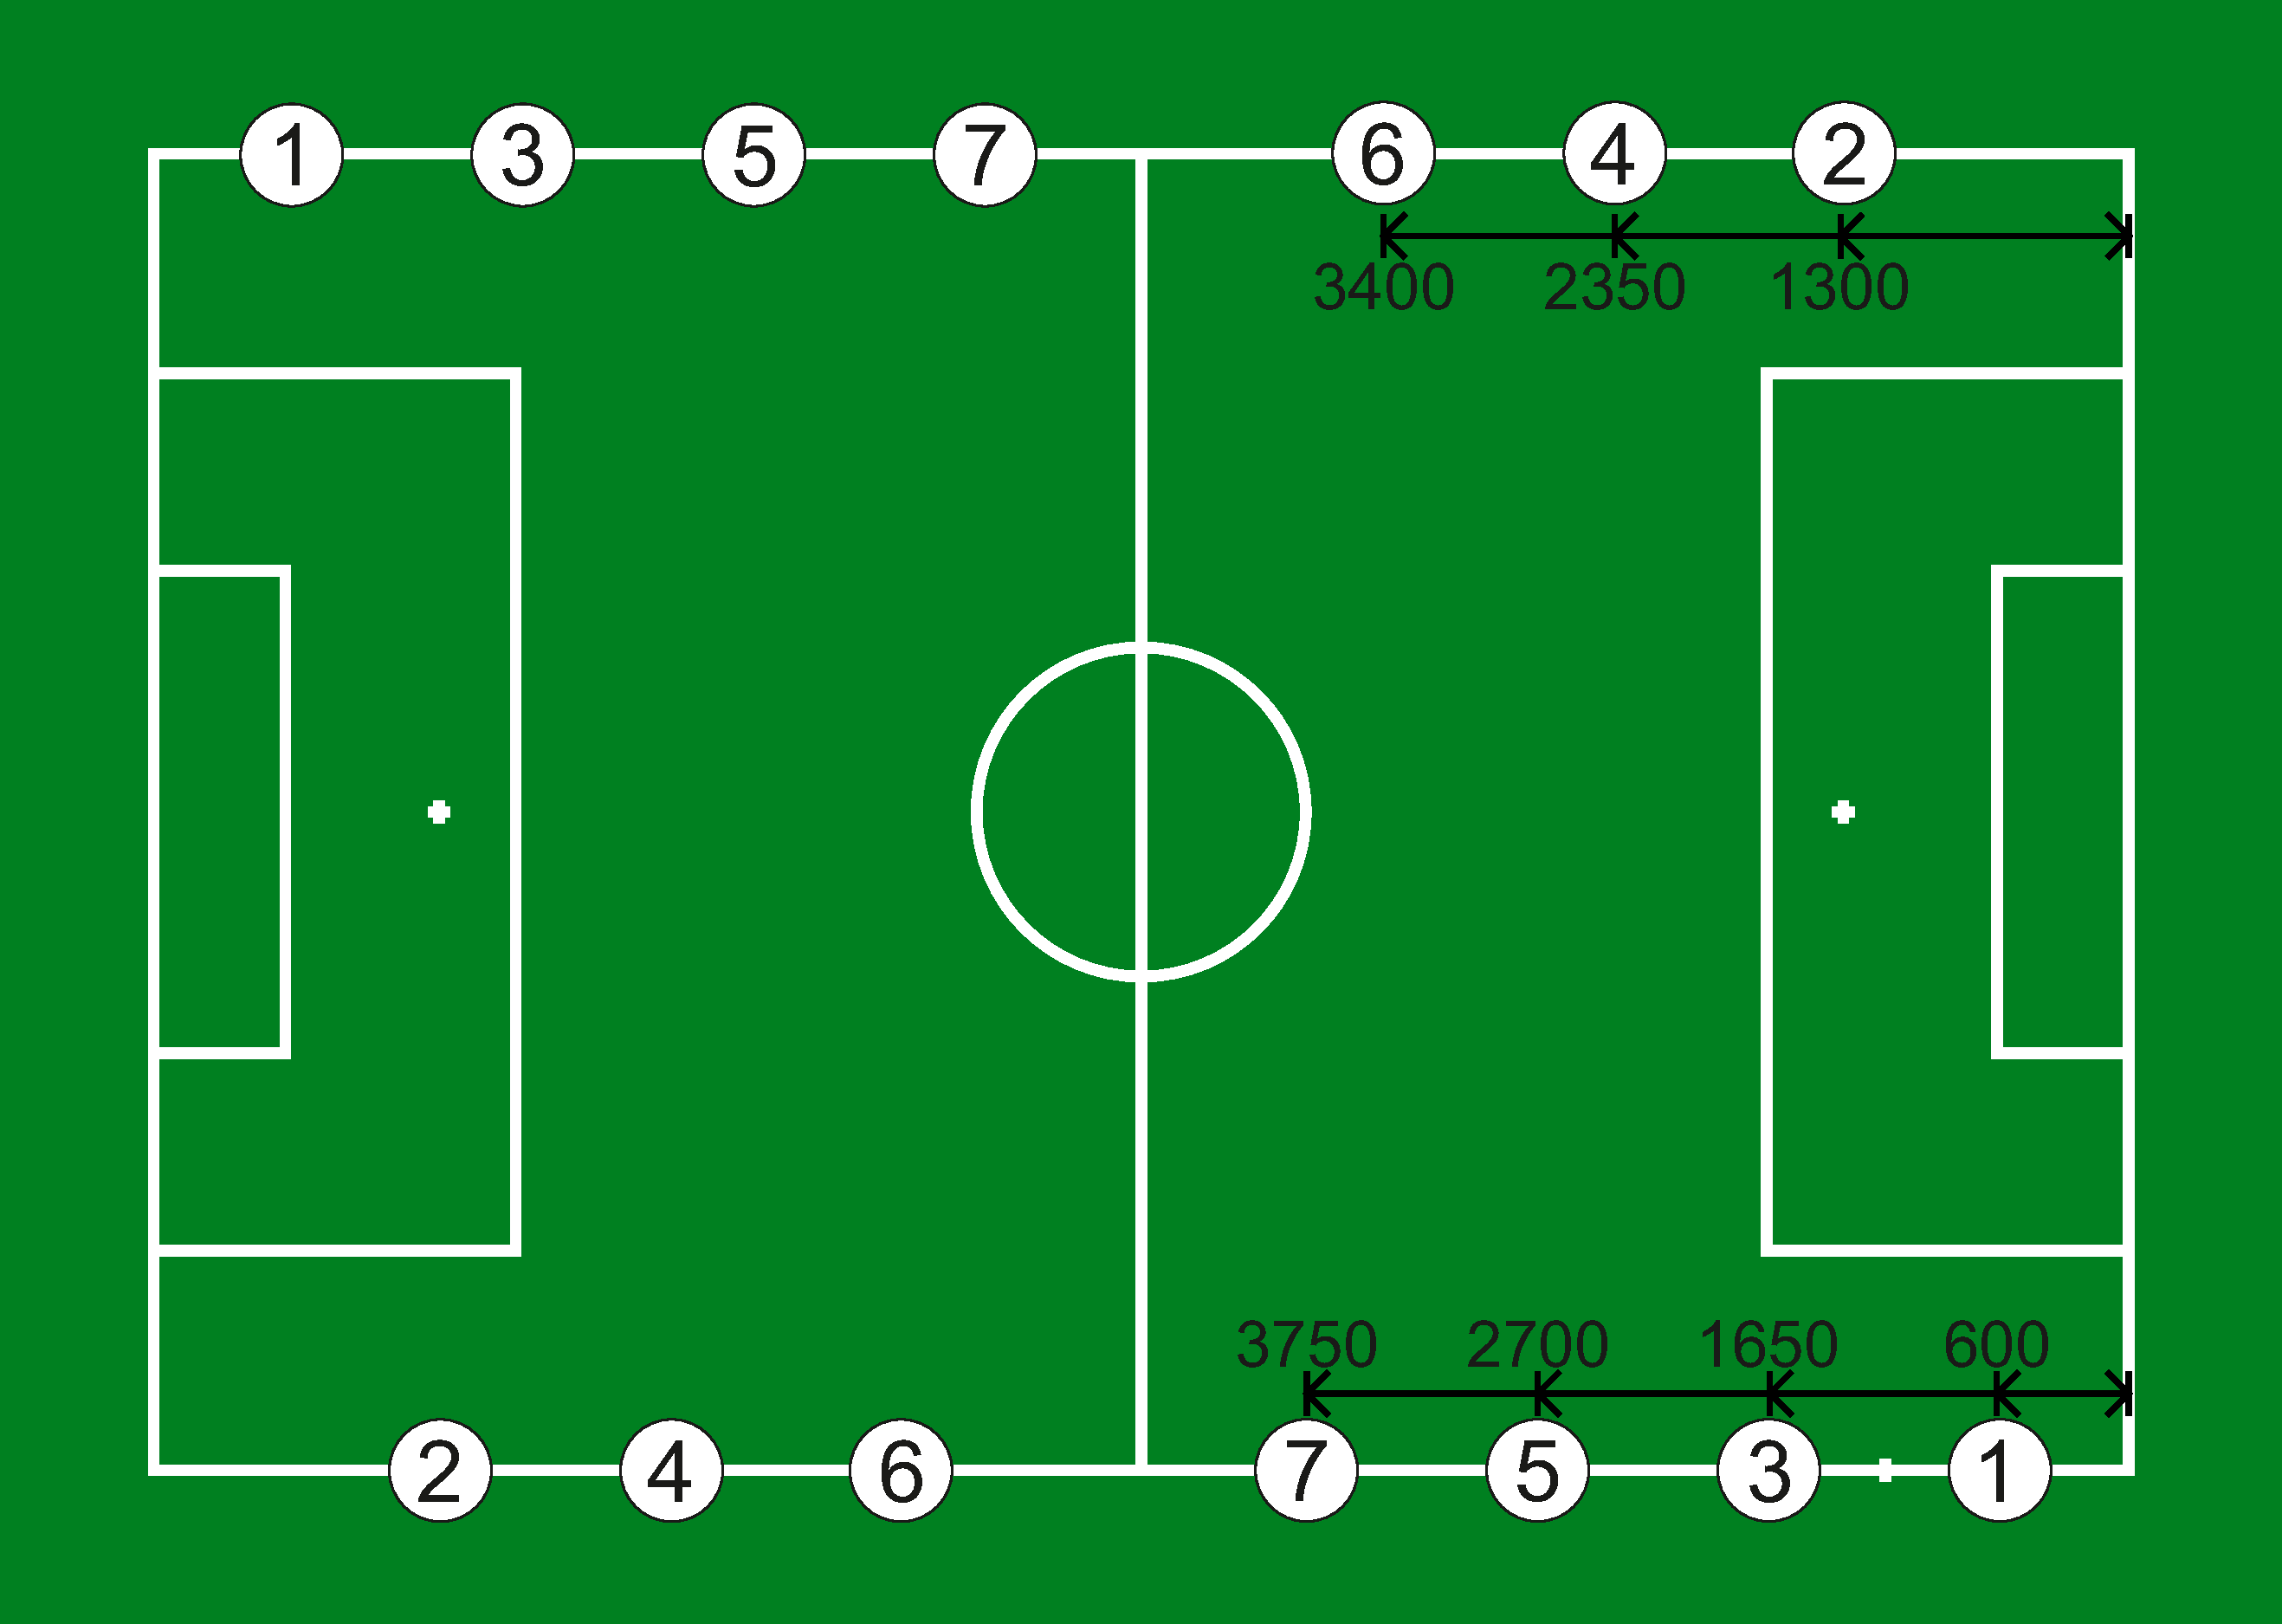
\includegraphics[width=1\columnwidth]{figs/initial_positions_7vs7.pdf}
            		\caption{Positions, player numbers and distances from the center of the goal line for the initial kick-off of the 7 vs. 7 robots.}
            		\label{fig:initial_positions_7vs7}
            	\end{center}
            \end{figure}
            Blue and red jerseys with numbers from 1 to 7 are provided by the OC/TC. If a team decides to play with own jerseys, they have to provide an additional one of the same shape. 

        \paragraph{WiFi}
            The available Wifi package budget defined in \cref{sec:wireless} will be increase by \qty{40}{\percent} both for the initial budget and for the budget for playing time extensions.  

        \paragraph{Referees}
            \label{sec:7vs7:referee}
            All referees are allowed to prevent robots from crashing to the ground by catching them beforehand and then laying them down gently. Additionally, the head referee decides whether a robot excessively damages itself and should remove it from the field via a forced ``Request for Pick-up'', \cf \cref{sec:request_for_pickup}.

        \paragraph{Robot Pool}
            Each team has to contribute at least 3 robots to the robot pool, \cf \cref{sec:7vs7:condition_for_participation}. If a team cannot provide enough own robots and there are still functional robots in the robot pool, then this team can get more than the 3 robots from the pool to restock up to 7 robots. However, the final decision is still up to the head referee. \\
            The robot pool exists only virtually, so that there is no central location where all pool robots are stored. Each team is also allowed to use their own pool robots when they are not in use. However, each pool robot gets a unique ID and in order to be able to recognize the pool robots visually, a sticker is attached to the outer sides of the upper arms and on the back of the head.

        \paragraph{USB logging}
            For logging, robots should work with both ext3 or ext4 formatted USB sticks. The USB stick should provide at least 8\,GB of free space.

        \paragraph{Robot Pool Evaluation}
            \label{sec:robot_pool_evaluation}
            In order to guarantee that the pool robots are functional, and all parts are working within their limits each team has to provide a proof of functionality one hour before a specific pool robot is planned for a game. Also, the team has to ensure that this robot had at least a cooldown period of \qty{15}{\minute} and is charged to at least \qty{80}{\percent}.
            A common robot evaluation image will be provided by the community with a standardized setup procedure (custom image) and with automatic calibration. Afterwards the robot should walk towards a ball and shoot it. If this evaluation is completed without any problems within \qty{2}{\minute} and the robot falls down less than 2 times, the evaluation is to be rated as functional. Otherwise, this robot is considered to be non-functional for the time being. Every team can propose such an image up to the 2022-06-01, as well as additional tests which should be included in such an evaluation image. A manual how to use the custom image should also be included.

        \paragraph{Hardware Related Penalties}
            \label{sec:7vs7:hardware_related_penalties}
            Since teams are partially playing with robots from other teams, there is a maximum of two hardware related penalties for each robot in the first half and one more in the second half.
            Hardware related penalties are:
            \begin{itemize}
                \item fallen robot or inactive robot, \cf \cref{sec:fallenrobots}
                \item request for pick-up in the playing or ready state -- either by the team or forced by the head referee, \cf \cref{sec:request_for_pickup} and \cref{sec:7vs7:referee}.
            \end{itemize}
            These penalties are counted by the GameController operator and after that a robot with additional hardware related penalties is excluded for the rest of the game (they are transitioned into the unstiffed state by the assistant referees, \cf \cref{sec:robot_states})!

        \paragraph{Own Pushing}
            In addition to the normal pushing rules, \cf \cref{sec:player_pushing}, pushing may now occur between any robots, i.e., also between teammates.

        \paragraph{Limited Diving}
            Pool robots are not allowed to dive for the ball on purpose, \cf \cref{sec:fallenrobots}, except for penalty kicks! In case of violation, the infringing robot will be taken out according to the forced ``Request for Pick-up'' rule, \cf \cref{sec:7vs7:referee}, and therefore counts as a hardware related penalty, \cf \cref{sec:7vs7:hardware_related_penalties}. However, this restriction does not apply to the team's own robots.

        \paragraph{Match Phases}
            Each match consists out of the following phases:
            \paragraph{Robot check} Each team marks and checks its robots sent to the robot pool as described in \cref{sec:robot_pool_evaluation} and reports its availability (1.5 hours before a match starts).
            \paragraph{Setup} One hour before the match starts, the teams receive their randomly selected robots. They have now time for set-up and calibration. For calibration only one half of the field is available for a team. The area within the center circle is not allowed to be entered by the robots until the match starts.
            \paragraph{Game} During a match additional rules apply for the pool robots. Referees are asked to try to save the robots' hardware by catching them before they crash onto the ground.
            \paragraph{After game} Teams have time of \qty{15}{\minute} to return the pool robots to the pool.

        \paragraph{Mode}
            The mode will be determined after teams have registered. At least 4 teams should register, before the challenge will be executed. The selected mode (e.g., group phase, double elimination, Swiss system tournament) will be determined after teams have registered.

\subsection{Visual Referee Challenge}

    \subsubsection{Challenge Goal}

        In the current SPL rules, the only time that a robot is required to listen directly to the human referees is for the kick-off whistle. Otherwise, all human referee decisions are communicated to the robots via electronic GameController messages. In moving towards the 2050 RoboCup goal, robots will need to directly interpret referee calls and signals (such as whistles, spoken calls and hand signals), rather than receive information from an external electronic source.
        
        This technical challenge tests a robot's ability to identify three categories of hand signals:
        \begin{enumerate}
            \item Static hand signals with one hand.
            \item Static hand signals with two hands.
            \item Dynamic (motion) hand signals with one or two hands.
        \end{enumerate}
        
        The intent of this challenge is to choose a \emph{subset} of potential referee calls in SPL games and test ability of a robot to recognise different types of hand signals in preparation for adoption in RoboCup games, rather than compile a complete set of all referee signals.

    \subsubsection{Challenge setup}

        One robot of the challenged team is placed in the center circle facing the head referee, standing upright (stiffened) with both hands by its side. The robot should be running in the challenge mode at the start of the challenge. The team is free to choose how the software is started.
        
        The head referee must stand on the T-junction of the center field line, opposite to the GC. The referee must wear a ``black-and-white'' stripped referee jersey (if available) and must  wear red gloves. The purpose of this clothing is to clearly distinguish the referee and their hands from background people. 
        
        The description of this challenge (and hand-signals) is described based on the viewpoint of the head referee. In these descriptions the ``red team'' is defined as playing from left-to-right, and the ``blue team'' as playing from right-to-left. The use of colours for identifying teams is used to give equivalence to the head referee calls during SPL games.
        
        The general procedure is as follows:

        \begin{enumerate}
            
            \item The referee selects a hand-signal (and direction where applicable).
            \item The referee blows the whistle once. The referee may use one hand to hold (and blow) the whistle. The referee may instead leave the whistle held in their mouth without their hands.
            \item \qty{1}{\second} after blowing the whistle, the referee indicates the hand-signal for \qty{10}{\second}.
            \item During that time or within an additional \qty{10}{\second}, the robot must indicate the hand-signal that it has identified by:
            \begin{enumerate}
                \item Using its hand(s) to \emph{mirror} the referee's signal. That is, if the referee given a signals for a decision for the ``red team'' using their right hand, the robot should \emph{mirror} this signal using the robot's \emph{left hand}, as the robot is facing the referee.
                \item Providing an audio phrase the referee's decision, e.g., ```Goal Red Team'''.  The exact wording is up to the team, but should clearly identify the referee's signal.
                \item (Optional), At the discretion of the GC/TCM developers, TCP messages may also be sent and interpreted to display the outcome of the robot's decision, however, this is not a requirement for the execution of the challenge.
            \end{enumerate}
            \item The length of time taken for the robot to indicate it's interpretation from the referee blowing the whistle is measured (rounded-up to the nearest second).
            \item If the robot cannot identify the signal, it should remain motionless and provide no audio output. A robot may continue to pose in the same position as the identified last signal.
            \item While not providing a hand-signal or using the whistle, the head referee must keep both hands flat and motionless by their side.
        \end{enumerate}

        This procedure will be repeated \textit{five} times. The referee should choose 2 one-hand static signals, 2 two-hand static signals, and 1 dynamic signal. Within each type, the referee randomly chooses a hand-signal and direction.The same hand-signal may be chosen twice (with different directions).

    \subsubsection{Available Hand-Signals}

        Each hand-signal for the challenge is described and pictured. Note that for the purpose of clarity, these do not necessarily correspond to human soccer hand-signals.

        \begin{itemize}
            \item \textbf{Kick-in \textlangle{}colour\textrangle{} Team.}
            One-handed signal. One arm, extended horizontally in the direction of the half of the field corresponding to the team that receives the Kick-in Free Kick. That is, right arm extended for the ``Blue team'', and left arm extended for the ``Red team''. The non-signal hand is flat and motionless by the side of the body.
%            \begin{figure}[ht!]
%                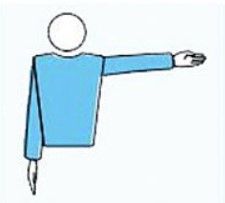
\includegraphics{figs/kick-off_referee.jpg}
%            \end{figure}
            \begin{figure}[ht!]
                \centering
                \begin{subfigure}{.33\textwidth}
                  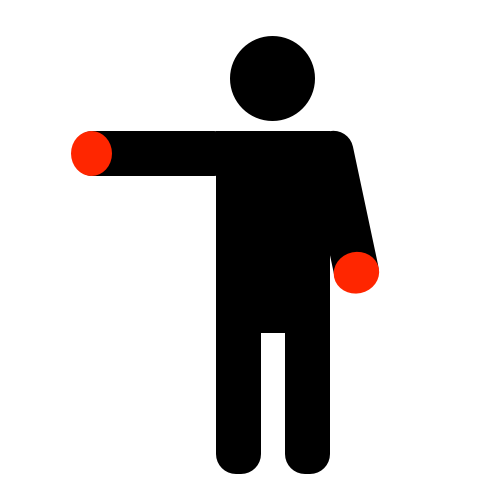
\includegraphics[height=120px]{figs/referee-signals/kick-in.png}
                \end{subfigure}
                \begin{subfigure}{.33\textwidth}
                  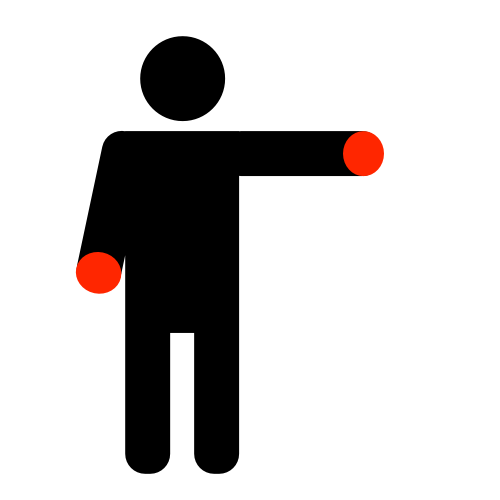
\includegraphics[height=120px]{figs/referee-signals/kick-in-flipped.png}
                \end{subfigure}
            \end{figure}
            
            
            \item \textbf{Goal Kick \textlangle{}colour\textrangle{} Team.}
            One-handed signal. One arm, extended 45-degree \emph{up} in the direction of the end of the field where the goal kick will occur. That is, right arm extended for the ``Blue team'', and left arm extended for the ``Red team''. The non-signal hand is flat and motionless by the side of the body.
            \begin{figure}[ht!]
                \centering
                \begin{subfigure}{.33\textwidth}
                  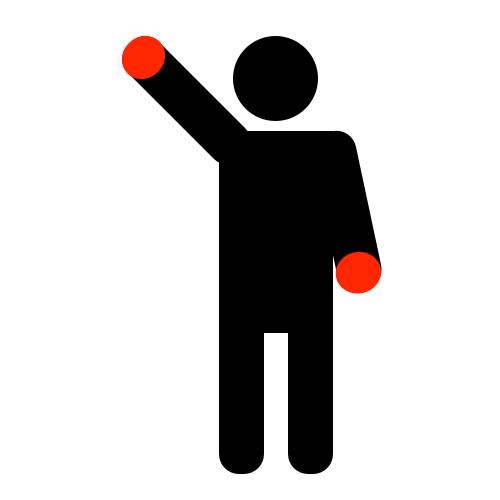
\includegraphics[height=120px]{figs/referee-signals/goal-kick.png}
                \end{subfigure}
                \begin{subfigure}{.33\textwidth}
                  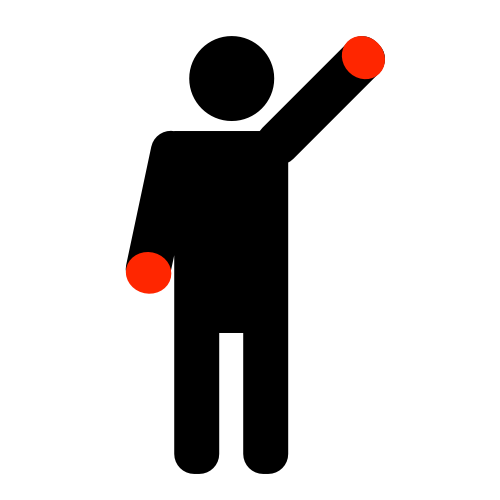
\includegraphics[height=120px]{figs/referee-signals/goal-kick-flipped.png}
                \end{subfigure}
            \end{figure}


            \item \textbf{Corner Kick \textlangle{}colour\textrangle{} Team.}
            One-handed signal. One arm, extended 45-degree \emph{down} in the direction of the end of the field where the corner kick will occur. That is, right arm extended for the ``Red team'', and left arm extended for the ``Blue team''. The non-signal hand is flat and motionless by the side of the body.
            \begin{figure}[ht!]
                \centering
                \begin{subfigure}{.33\textwidth}
                  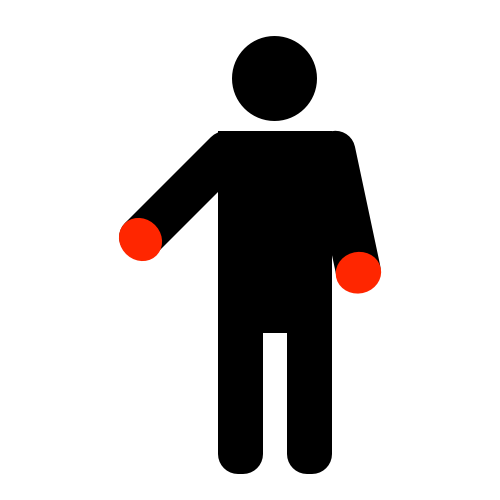
\includegraphics[height=120px]{figs/referee-signals/corner-kick.png}
                \end{subfigure}
                \begin{subfigure}{.33\textwidth}
                  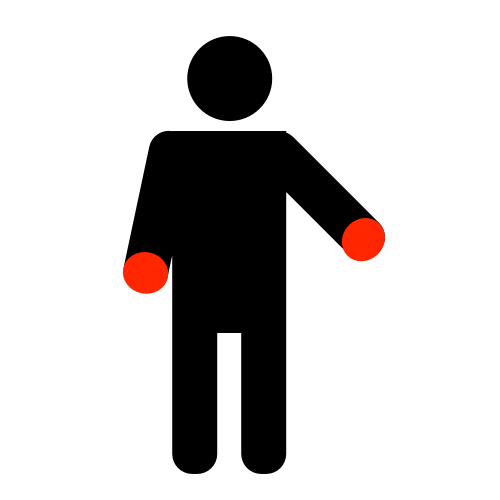
\includegraphics[height=120px]{figs/referee-signals/corner-kick-flipped.png}
                \end{subfigure}
            \end{figure}
            

            \item \textbf{Goal \textlangle{}colour\textrangle{}  Team.}
            Two-handed signal. One arm, extended pointing at the center circle. One arm, extended horizontally in the direction of the half of the field corresponding to the team that scored the goal. That is, right arm extended for the ``Blue team'', and left arm extended for the ``Red team''.
            \begin{figure}[ht!]
                \centering
                \begin{subfigure}{.33\textwidth}
                  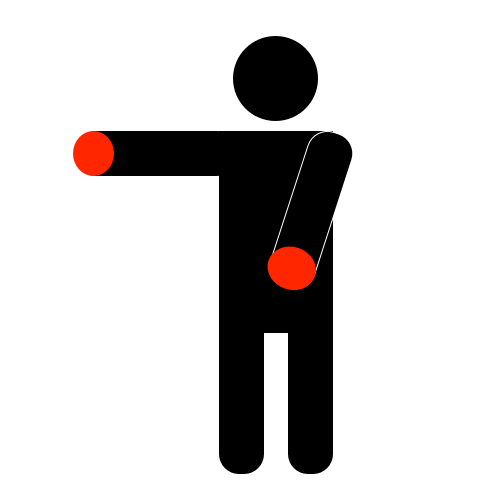
\includegraphics[height=120px]{figs/referee-signals/goal.png}
                \end{subfigure}
                \begin{subfigure}{.33\textwidth}
                  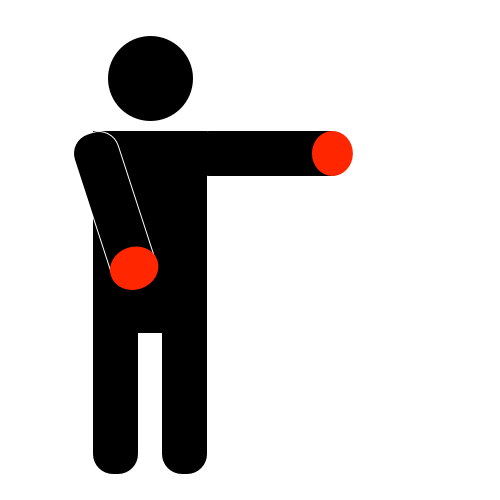
\includegraphics[height=120px]{figs/referee-signals/goal-flipped.png}
                \end{subfigure}
            \end{figure}


            \item \textbf{Pushing Free-kick \textlangle{}colour\textrangle{}  Team.}
            Two-handed signal. One arm, vertical with bent elbow and palm facing in the direction of the extended arm. One arm, extended horizontally in the in the direction of the half of the field corresponding to the team that is \emph{given} the penalty. That is, right arm extended for the ``Blue team'', and left arm extended for the ``Red team''.
            \begin{figure}[ht!]
                \centering
                \begin{subfigure}{.33\textwidth}
                  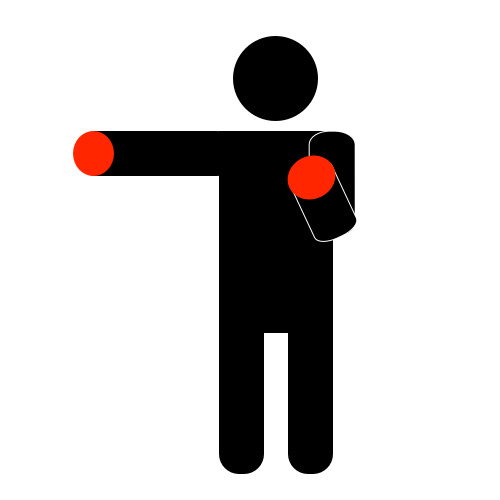
\includegraphics[height=120px]{figs/referee-signals/pushing.png}
                \end{subfigure}
                \begin{subfigure}{.33\textwidth}
                  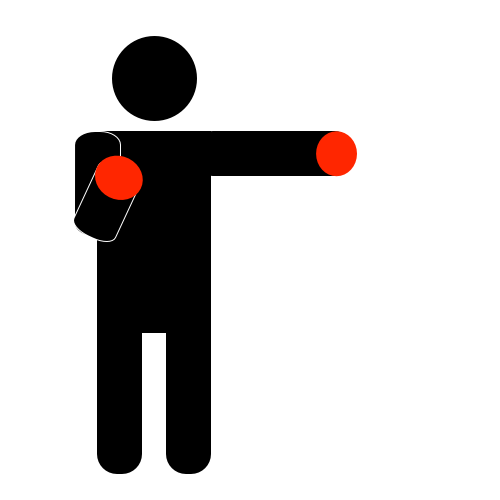
\includegraphics[height=120px]{figs/referee-signals/pushing-flipped.png}
                \end{subfigure}
            \end{figure}

            \item \textbf{Full-Time.}
            Dynamic two-handed signal. Both arms slowly move symmetrically inward and outwards on a horizontal plane, bending at the elbows. Note, for the purpose of this challenge, the whistle associated with this signal should be a \textit{single} blow, unlike in normal SPL games.
            \begin{figure}[ht!]
                \centering
                \begin{subfigure}{.33\textwidth}
                  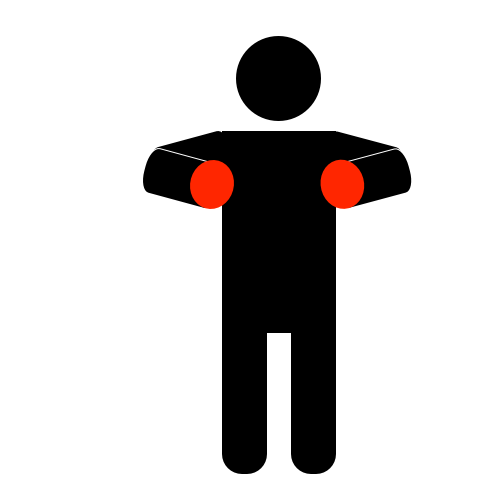
\includegraphics[height=120px]{figs/referee-signals/full-time-start.png}
                \end{subfigure}
                \begin{subfigure}{.33\textwidth}
                  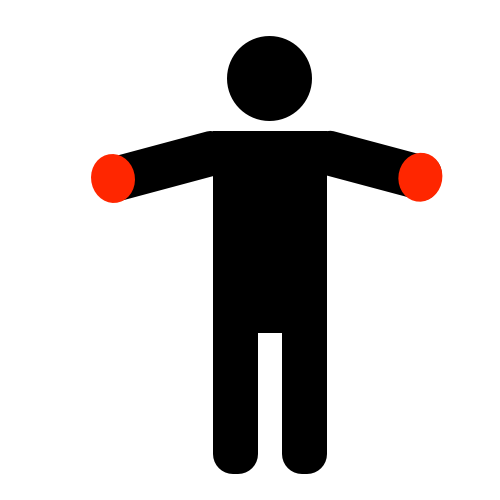
\includegraphics[height=120px]{figs/referee-signals/full-time-end.png}
                \end{subfigure}
            \end{figure}

        \end{itemize}

    \subsubsection{Challenge evaluation}
        A team scores 1 point for every hand-signal that is correctly identified. A team score an additional 1 point for correctly identifying the team corresponding to the signal (where appropriate). A team looses 1 point for incorrectly identifying a hand-signal (note a team may have a negative final score). The total time for the robot to identify each hand-signal is summed (If a robot fails to identify a hand-signal the time for the hand-signal is \qty{10}{\second}. If a robot incorrectly identifies a hand-signal, the time is how long the robot took to provide the incorrect identification).
    
        Teams are ranked by their total points. In the event of tie-breaks, the team with the fastest total time to identify all hand-signals is ranked higher. The team with the highest total points, and lowest total time (for tie-breaks), wins the challenge. 

\subsection{Dynamic Ball handling Challenge}

    This challenge extends the idea of RoboCup 2021's Passing Challenge. The purpose of this challenge is to enhance skills in ball passing and handling, and in robot's movement estimation.

    \subsubsection{Challenge Goal}

        Score as attacking team a goal after a double pass without letting the defending players touch the ball.

    \subsubsection{Challenge Setup}

        This challenge uses a standard SPL field, with GameController and 3 attacking robots provided by the challenged team and three defending robots operating a provided common image (see \cref{sec:Challenge_image}) from another team. If more than one image exists, than multiple images will be provided and for each run a new one will be randomly selected.

        Attacking teams have to have their robots ready \qty{40}{\minute} before a run starts. Attacking robots are not allowed to be changed afterwards. Then the defending teams receive which randomly selected common image will be used. In that time the defending robots have to be flashed and calibrated.

        Since the challenge has three runs for each team, each team will be teamed with another team for a run. Both teams have to provide the same three robots (except one robot breaks) as attacking as well as defending team. Following from this each run is divided into two parts. Executed after each other.

        The robots are placed by the referees with some randomness to left or right as follows:

        \begin{description}
            \item[Attacker:] 1st: goal area front line (Player No 1); 2nd: next to center line left of center circle (Player No 2); 3rd: next to center line right of center circle (Player No 3).
            \item[Defender:] 1st: within center circle (Player No 3); 2nd: front line penalty area (Player No 2); 3rd: goalkeeper in the middle between the two goal posts (Player No 1). Defending robots are limited to a maximum speed of \qty{20}{\cm \per \second}.
            \item[Ball:] On penalty spot of the attacking team's side
        \end{description}

        \begin{figure}[t!]
            \begin{center}
                \leavevmode
                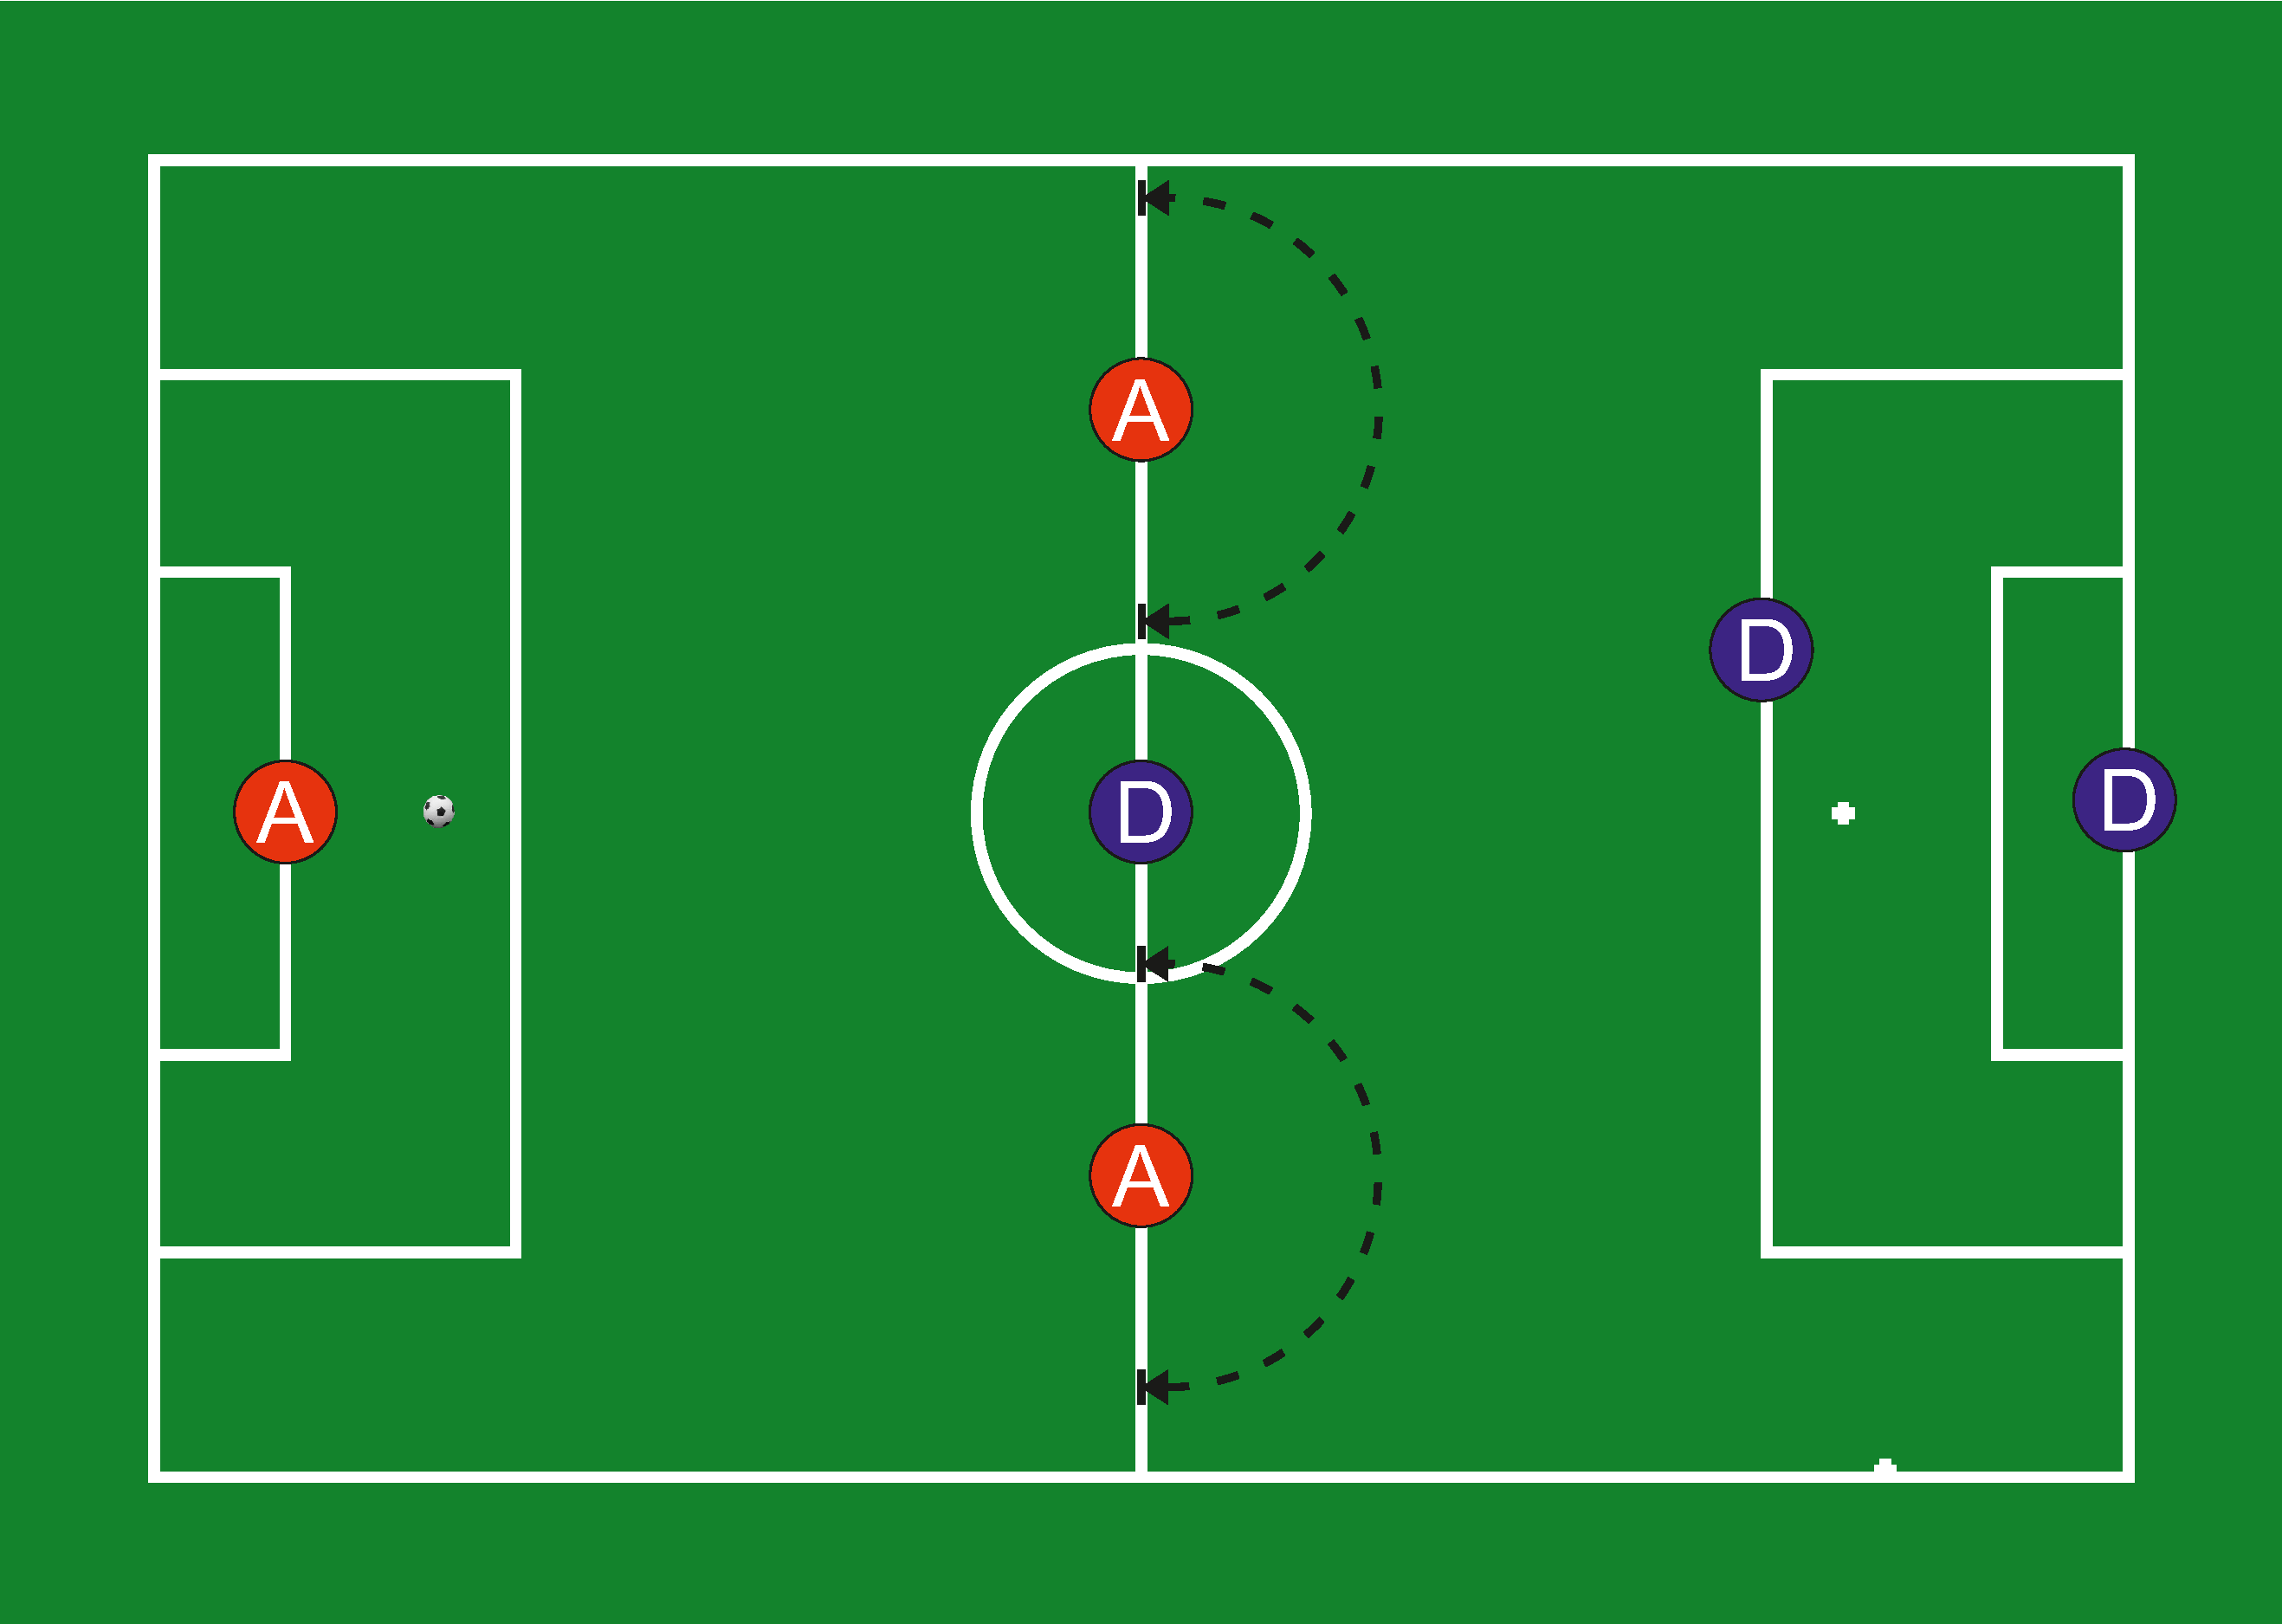
\includegraphics[width=1\columnwidth]{figs/ball_handling_positions.pdf}
                \caption{Possible positions of the attacking (red) and defending (blue) robots at the beginning of the challenge. The black semicircle indicates the area in which a pass is valid.}
                \label{fig:ball_handling_positions}
            \end{center}
        \end{figure}

    Each team has three attempts to run this challenge.

    \subsubsection{Challenge Execution}

        All six robots have to be in the Wi-Fi. In \texttt{initial} the robots get placed at their randomized starting positions. GC goes from \texttt{ready} directly into \texttt{set}. The ball gets placed, and the head referee starts the challenge execution with one whistle, like at kick-off. If a robot does not listen to the whistle, it will get the delayed \texttt{playing} signal from the GC.

        In \texttt{playing} the following happens: The 1st attacker plays the ball towards the 2nd or 3rd attacker while he is under attack by the 1st defender.
        A pass counts as a valid pass if the ball stops in front of the receiving robot towards the opponent's goal. The ball has to stop in the vicinity of the receiving robot (at max \qty{1}{\metre} distance between receiver and ball, see~\cref{fig:ball_handling_positions}).
        The 1st defender does not walk back in its own half and the goalkeeper remains on the goal line and is not allowed to dive. The objective of the defending team is to intercept the passes, see stopping criteria.

        After the 2nd or 3rd attacker received the ball, and the ball is in the defender's half, it gets attacked by the 2nd defender. The task of the 2nd or 3rd attacker is now to pass towards the 3rd or 2nd attacking robot, which than shots onto the goal.

        If a defender pushes an attacking robot, the attacking team gets a time bonus of \qty{15}{\second} and the pushing robot will be removed from this run.

    \subsubsection{Challenge Scoring}

        For each run the referee measures the execution time from initial whistle until the run is stopped by one of the following criteria:

        \begin{itemize}
            \item A defender touches the ball.
            \item Ball leaves the field.
            \item An attacker pushes.
            \item A run exceeds \qty{4}{\minute} execution time.
            \item A goal is scored.
        \end{itemize}

        A score for the run will be calculated based on the following rules:

        \begin{enumerate}
            \item The time measured counts.
            \item If an attacking robot has been pushed by a defender, subtract \qty{15}{\second}.
            \item If a goal has been scored after two passes, subtract \qty{30}{\second}.
            \item If a ball has been passed wrongly, add \qty{10}{\second} for each incorrect pass.
            \item If the ball got touched by the 1st or 2nd defender, execution time will be \qty{240}{\second}.
            \item If the ball leaves the field not from inside the defending goal area, execution time will be \qty{240}{\second}.
            \item If an attacking robot has pushed, execution time will be \qty{240}{\second}.
        \end{enumerate}

        The final result is the mean time out of three runs.

    \subsubsection{Challenge image}
        \label{sec:Challenge_image}
        A common image will be provided by the community with the standardized setup procedure and with automatic calibration. Every team can propose such an image until 2022-03-15. The image will be tested until 2022-03-31 if they match the requirements and afterwards published if not the team gets feedback and has the opportunity to hand in a revised image.

        \begin{enumerate}
            \item One image applying to the standard button interface, using autonomous calibration and receives it player number through a text file on USB-stick.
            \item Existence of documentation on how to flash, how to operate a robot, how to handle issues.
            \item Does it apply to the rules?
            \item Does it operate robustly?
            \item Does it attack according to the rules?
        \end{enumerate}

\subsection{Open Research Challenge -- Video analysis / statistics}
In order to evaluate the progress of the league, regardless of the annual rule changes, we need statistics similar to human soccer. Therefore, only GameController/TeamCom statistics are not sufficient for this. That's why there is an Open Research Challenge, as already known from the year 2019 (and previously until RoboCup 2014), which will focus on the generation of statistics from external video data from a go-pro type camera viewpoint.

    \subsubsection{Challenge Goal}
    For this Open Research Challenge two major goals exist. The more short-term goal is to calculate extrinsic camera parameters (camera matrix) from the camera feed and to locate/track all moving objects (ball, robots) on the field. In addition to this, the more long-term goal involves the creation of game statistics based on the located objects and positions from the short-term goal. Here, the following statistics, among others, might be of interest, such as time under control, shots on goal (successful/unsuccessful), passes and so on. Since this is an open challenge, the decision of what to show (short-term, long-term, parts of it) is, within the scope of the goals aforementioned here, entirely up to the teams. In addition, the execution time for this challenge is also not relevant for the time being whether you process it online or offline to the video stream.

    \subsubsection{Condition for participation}
    \begin{itemize}
    \item In order to compete in this Challenge, teams must notify the TC (\url{rc-spl-tc@lists.robocup.org}) of their interest in participating by 2021-12-31, at the latest.
    \item Subsequently, all participating teams will receive a pre-processed video from the RoboCup2019 (i.e. a sequence of images) and have to label it according to the enclosed instructions. Annotating must be completed by 2022-02-01 in order to form a shared ground truth data set. The exact details are given to the teams together with the to be labeled data set.
    \item The annotations should be saved and uploaded as a single file per image sequence (so only one file per participating team) in the CSV format where the columns must be as follows:    

    \hfill{}%
        \begin{tabular}{|c|c|c|c|c|c|c|c|}
        \hline 
        \textbf{filename} & \textbf{label} & \textbf{x\textsubscript{min}} & \textbf{y\textsubscript{min}} & \textbf{x\textsubscript{max}} & \textbf{y\textsubscript{max}} & \textbf{jersey color} & \textbf{jersey number}\tabularnewline
        \hline 
        \hline 
        test.jpg & 0 & 0 & 0 & 1919 & 1079 & 0 & 100\tabularnewline
        \hline 
        test.jpg & 1 & 300 & 300 & 400 & 400 & -1 & -1\tabularnewline
        \hline 
        $\ldots$ & $\ldots$ & $\ldots$ & $\ldots$ & $\ldots$ & $\ldots$ & $\ldots$ & $\ldots$\tabularnewline
        \hline 
        \end{tabular}
    \hfill{}
    \vspace{0.25cm}\\
    Thus this CSV file would look like that:\\
    \hspace*{0.8cm}\texttt{test.jpg,0,0,0,1919,1079,0,100}\\
    \hspace*{0.8cm}\texttt{test.jpg,1,300,300,400,400,-1,-1}
    \item With this shared ground truth data set, teams can then implement their own approach/ideas. Also any failures in the annotations can be corrected by the community/teams since the data will be shared on the SPL Github\footnote{https://github.com/RoboCup-SPL}.
    \item The teams have to create a poster (A3 or A2 size) for the RoboCup 2022 showing their results and prepare a short 3 minutes oral presentation which additionally explains and shows the idea and results of this approach. If there is a GameState monitor on site, it can be used for a presentation. However, this depends on the location and the teams should be prepared to give their presentation only with their poster if necessary.
    \item All teams are requested to publish the code for their approach to enable a fast progress of the league in this area. However, only the top 3 ranked teams are required to publish their code with instructions within one month after the RoboCup 2022.
    \end{itemize}

    \subsubsection{Scoring}
    The winner will be decided by a vote among the SPL teams using the Borda count mechanism (\url{http://en.wikipedia.org/wiki/Borda_count}). Each participating SPL team will vote for their top 5 teams in order (excluding themselves).\\ 
    Teams are encouraged to evaluate the performance based on the following criteria: 
    \begin{itemize}
        \item Achievement of the long/short-term goal,
        \item execution time (and hardware requirements),
        \item metrics (accuracy/precision/recall),
        \item technical strength and
        \item novelty.
    \end{itemize}
    At a time decided by the designated referee, within one hour of the last demonstration if not otherwise specified, the captain of each team will submit the team's rankings by filling out an online form. Any points awarded by a team to itself will be disregarded. The points awarded by the teams will be summed and thus form the score of this challenge which is then converted according to the formula described in the beginning of this section.

    \subsubsection{Labelling}
    This section gives a brief overview of the labelling task.\\

    Input data (given):
    \begin{itemize}
        \item The assigned, pre-processed, go-pro videos/sequences from a game of the RC2019. These are not whole halftimes but only an excerpt of 5000 frames (at 30FPS this means about 2:42 min of continuous playing time). 
        \item Additionally the GameController data, TeamCom logs and the intrinsic parameters of the go-pro are given.
    \end{itemize}

\urldef\colortable\url{https://github.com/RoboCup-SPL/GameController/blob/RoboCup2021/include/RoboCupGameControlData.h#L15}

    Output data (to be annotated):
    \begin{itemize}
        \item Labelling of all robots participating in the game and the (main) ball: These objects should be labeled using bounding boxes, characterized by the top-left and bottom-right corner. Special attention should be paid to the bottom edge as this will be used to determine the position of the object.
        \item In addition, the robots must be labeled with their jersey color (as number based on the GC assignment\footnote{\colortable}) and jersey number. However if the jersey number is not identifiable an ID starting with the number 100 and upwards should be used instead to clearly identify this robot in the sequence. \\
        \textit{Note:} It could happen that you can't identify a robot and therefore give it an unique ID $\geq$100 and later you see its player number. Then this robot should also get its jersey number retroactively for all previous frames instead of the ID $\geq$100.
    \end{itemize}
    The calculation of the extrinsic camera parameters (camera matrix) is optional.
%Preferably for each frame, although this is mainly necessary when the camera was moved/wobbled. However, it should be checked at least once for each minute whether the camera matrix is still appropriate.

    Also not everything is fixed yet so that the TC is happy to accept suggestions at \url{rc-spl-tc@lists.robocup.org}.
